\begin{block}{case study: norfolk, va}
    We model a \emph{hypothetical} house in Norfolk, VA, where sea level rise drives nonstationary future flood hazard, following the approach of \cite{zarekarizi_suboptimal:2020}.
    \begin{figure}
        \centering
        \includegraphics[width=\textwidth]{historic_surge.pdf}
        \caption{
            Time series of annual maximum of storm surge (after subtracting mean sea level) at Sewells Point, VA (NAVD datum).
        }
        \label{fig:observations}
    \end{figure}
    \begin{figure}
        \centering
        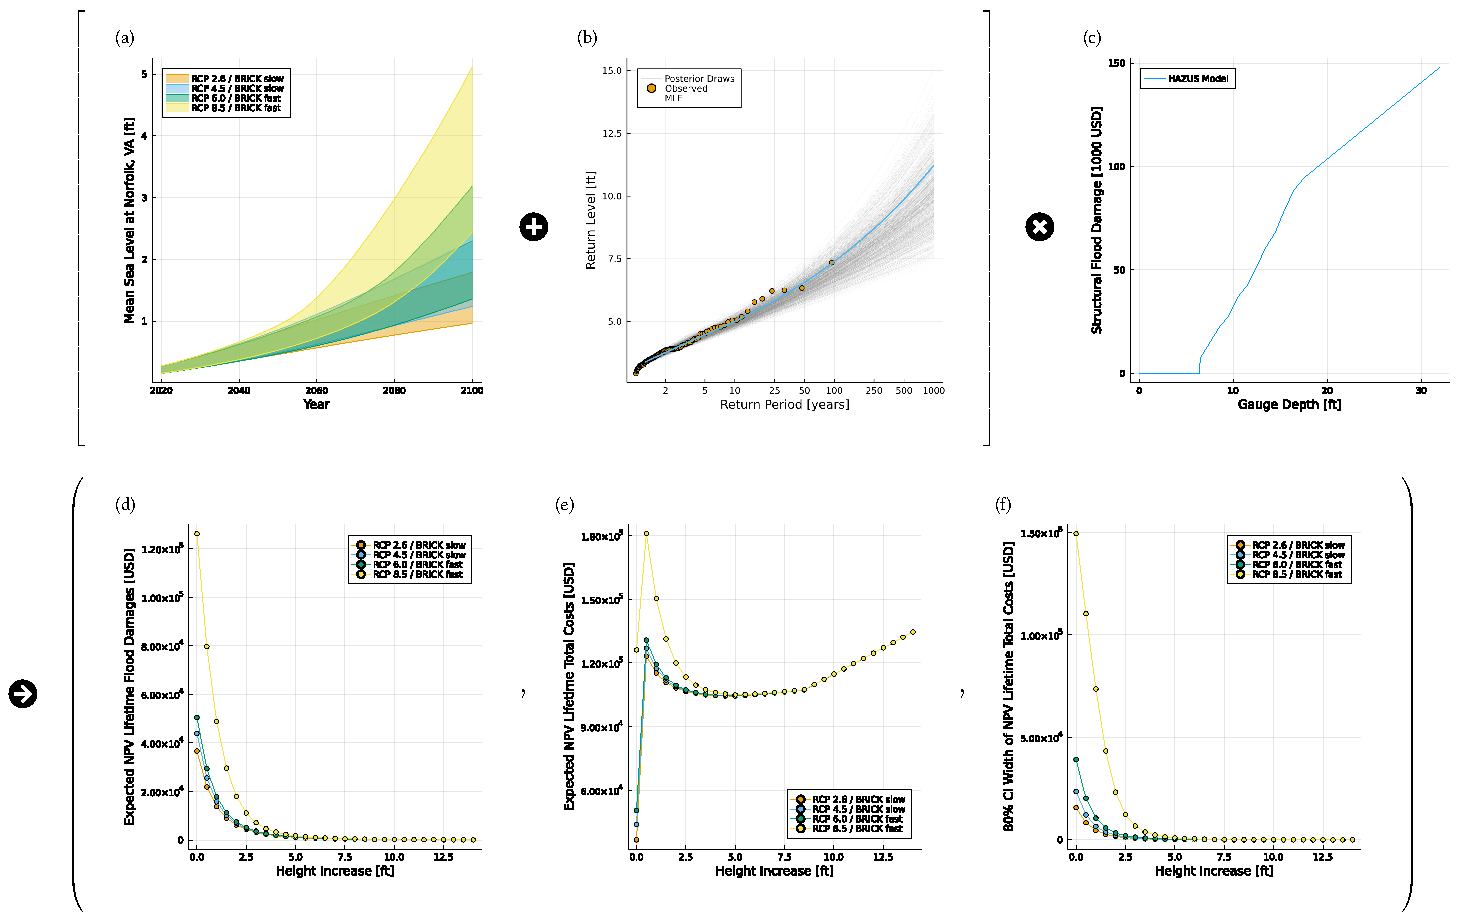
\includegraphics[width=\textwidth]{hazard-tradeoffs.pdf}
        \caption{
            Neglecting hydrodynamics, we add sea level rise (a; see ref.~\cite{ruckert_coastal:2019}) to a Bayesian GEV model of storm surge (b) to get flood hazard.
            The convolution of hazard and fragility (c; see ref.~\cite{zarekarizi_suboptimal:2020}) yields an assessment of damages and tradeoffs (\cref{fig:tradeoffs}).
        }
    \end{figure}
\end{block}